\chapter{Developer documentation}
\label{ch:impl}

For this project a high level programing language was needed which can support dynamic typing for creating easy statements and storing
lot of different data, the language also has to support runtime interpretation so the user defined statements can be used without
creating a whole new programing language and compiler for it. For these reasons Javascript with the V9 was chosen. 

\section{Architectural Overview}

The toolkit is heavily depends on the libgit2 \cite(libgit2) library which is a portable, pure C implementation  if the Git core methods,
this library has a version for JavaScript and Node.js which is the nodegit \cite(nodegit).
The whole toolkit architecture can be represented with the following diagram:

\begin{figure}[H]
	\centering
	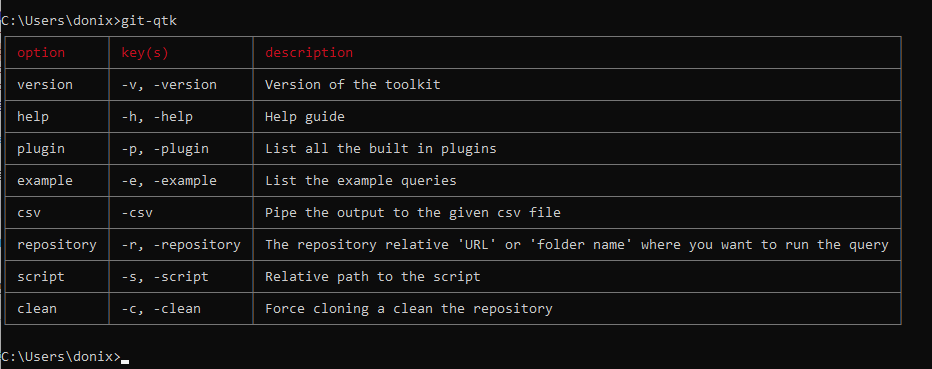
\includegraphics[width=350px]{help}
	\caption{TODO}
	\label{fig:fig-help}
\end{figure}

The \textit{Query} class is responsible to connect all the modules altogether and also for the IO operations. The query also also
responsible for reading the history from the repository and passing it to the plugins for parsing. The parse data will be stored
in the \textit{Database}. Before the parsing happens the input script also has to be recognized which is done by the \textit{Parse}
module. After both of them is ready the \textit{Runner} module will run the query based on the script and database.

\subsection{Database}

We need to somehow store all the data coming from the parser and plugins. We can assume that the plugins will reduce the size of the
pure data from the repository history. So to provide maxium performace for the query we can use an in-memory database. 
We can also assume that the database will be immutable after the parsing is done. 

The database is collections of hash maps based on the models. The hash map keys are defined by its model \textit{key()} method.
The reson behind this database structure is in the join mechanism in the query. The hash map is implemeted with the built in 
\textit{Map} \cite{map} which has a acceess time and space compexity of:

\( O(1) \)

In this way if we connect two models where at least of the models field is a key then we can assume that:\newline
If: N is the count of records by A model
	M  is the count of records by B model
\(O(N * M) = O(N)\)

\begin{figure}[H]
	\centering
	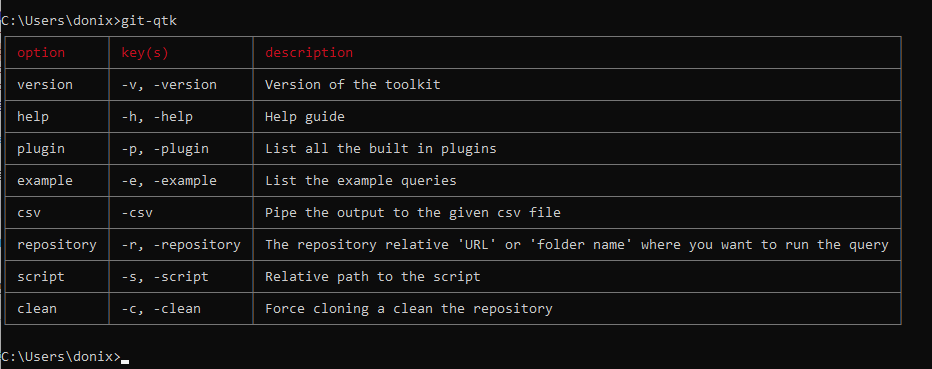
\includegraphics[width=350px]{help}
	\caption{TODO: databse mod}
	\label{fig:fig-help}
\end{figure}

\subsection{Extensions}

As discussed in the \nameref{Extending with plugins} are the way to add more features to extensions to the toolkit.
Let's look at the included basic \textbf{Git} plugin and its models \textbf{Commit}, \textbf{Author}, \textbf{File}.
This plugin will do the most basic parsing for the histroy which is to extract the commits, the authors, and the files
in the project.

What is needed to make a plugin:
\begin{itemize}
	\item \textit{init()} - The init will be called when repository is opened.
	\item \textit{parse(db, commit)} - This will be called for each commit, the database is expossed as a \textbf{Observer pattern}
	\item \textit{post()} - This will be called when all the commits are parsed
\end{itemize}

The commit in the \textit{parse(db, commit)} is defined in the libgit2 plugin.

The plugin also provided information about itself and what models brings to the database. 
The models will be loaded into database before \textit{init()} is called.

\subsubsection{Functions}

Functions are help for the user to predefine some often used functions for the given plugin.
For example: we may only need a short id for the commit so we can call \textit{short(sha)} inside our query expressions.
Behind the scene this will be injected into the sandbox where the expressions are evaluated.

To define a new functions just pass the function in an array in the \textit{functions()} method.

\subsubsection{Reductors}

Reductors are similar to Functions but its only can be used if a grouping is presented in the query. This will
run for each record in that group. The reductor should be a function and has 2 parameter \textit{reductor(acc, obj)}.
The acc will accumulate the result and the object will be the record itself.

To define a new reductor just pass the function in an array in the \textit{reductors()} method.

\subsubsection{Model}

A model is simply defining the structure of data it has two major function \textit{parse(input)}, \textit{parse(key)}. 
This will take the inputand transform it that way the database is storing them. 
\textit{name()} will be the name how it can be refered in the from tag.

Lets look at the Git plugin:

\lstinputlisting[caption={plugins/git.js}]{../plugins/git.js}

\subsection{Parsing and validating scripts}

(2)

\subsection{Parsing Git histroy}

breadth-first search (2)

\subsection{Running the query}

(2)

\section{Tools}

(1)

\subsection{Gitub}

\subsection{VS Code}

\section{Testing}

(0.5)

\subsection{Unit tests}

(2)

\subsection{Integration tests}

(2)

\chapter{Runtime measurement}
\label{appx:simulation}

(3)